\section{Origins of life}

Somehow, someway, we came from something and became this. The world around us and all the living things in it were not always so, and the amount of time that has passed since our planet was the new kid on the block is so astoundingly massive that we can’t really conceive it. This isn’t our fault - the biology of our particular form of life simply isn’t designed to mentally cross such vast gulfs of time. Naturally, then, knowing how it all began becomes quite difficult, and the only thing we can say for certain is that we don’t know for certain how it started.

We’ve made theories about this for a long time, and for most of that time those theories were founded in theology. If you went back in time and asked an Assyrian, she would claim that life originated from the great God-Emperor Ashur. You go forward in time a bit and ask the Greeks, and they’ll point you to the stars and the fathers of their Gods, the Titans. Go forward a bit more and you’ll hear Christians tell you that life was formed out of clay by Yahweh, after he had built the planet and given it light and water and all that. (Unless you’re a woman, in which case you were made out of a man’s rib. The sparerib theory?) 

\begin{center}
	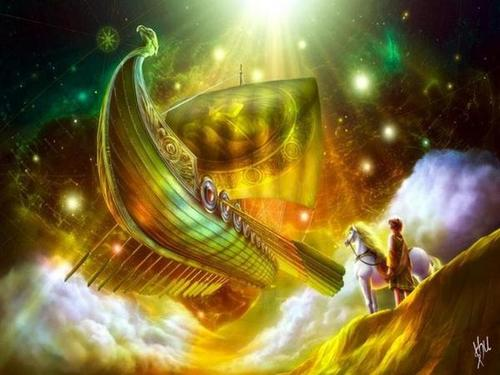
\includegraphics[width=0.45\textwidth]{magicship.jpg}
\end{center}

We’ve gotten a bit more methodical since then, and we know a bit more about the specifics of life, so we have constructed some better models. Modern, scientific theories have limited it to a narrow method involving RNA and interactions between chemical compounds in soups of primordial liquids. We know the basic ingredients to the recipe, but exactly how to cook is just theorized. We can line up all these ingredients in vials in a lab, walk down the line past them; all we need is water, specific monomers and minerals, and energy. Take a moment to consider how bizarre it is that given pressure and time, the contents of the vials have turned into beings capable of painting the Sistine chapel and landing robots on comets. From oozing, primordial goo to beings capable of producing masterworks of art and technology.

There are three different theories worth mentioning, and it also worth mentioning that they are theories, and not assertions of truth. The three theories are all pretty tasty; respectively the soup, pizza and sandwich theories. Let’s dig in:

\subsection{Soup}
(Kilde: common knowledge, burde kanskje finne en spesifikk kilde)
The soup theory is the first and most basic modern model of the origin of life on earth, and was formulated by the soviet biologist Alexander Oparin way back in 1924. It postulates[1] that (billions of years ago mind you) in the time when the planet was a toddler, the atmosphere was weaker and the elements on earth were more directly exposed to energy waves from space. This energy worked as a catalyst on simple chemical compounds - called monomers - which met for parties in the pools and eventually fused to create more complex compounds. With enough partying, these monomers turned into RNA, and the RNA eventually gave us photosynthesis and respiration, the two key ways lifeforms harvest energy. What we don’t know is how this fusion happened, and we don’t know how the RNA led to DNA. That’s it for starters, onwards to the main course, the pizza theory: 

1:  Shapiro, Robert (1987). Origins: A Skeptic's Guide to the Creation of Life on Earth. Bantam Books. p. 110. ISBN 0-671-45939-2.

\subsection{Pizza} (kilde: store kloke boken, get them details)
What separates the pizza from the soup is the spacial dimension. It’s very similar to the soup, but instead of large primordial pools, the pizza postulates that it is more likely that life originated in shallow basins of water near the surface. This gives two clear advantages over the soup; access to flat surfaces of rocks containing tasty minerals, and a closer proximity to the energy waves of the sun. This trifecta is a bit more proximate and powerful when in a shallow, ‘two-dimensional’ space, as the sun’s rays can hit both the monomers and the minerals and catalyze the partying between them all even more. There’s a problem with this theory too, however, and that is that it doesn’t explain how the earliest monomers got the right amount of water to form stable polymers. Science is smart, though, and since the pizza theory has some holes, a third theory has been presented, and like a sandwich, it involves layers. Enter the sandwich:

\subsection{Sandwich} (kilde, artikkel lagt ut av homeboy Kjell Morten, get details)
This theory is again similar to the others, but the difference here is the delivery mechanism of the catalyzing energy. This theory postulates that life may have begun in the tiny spaces between layers of the mineral mica - these spaces correspond precisely to the size of the earliest compounds (a single nanometer), and the layers of mica are so atomically flat that even the tiny DNA molecules show up as ridges on the surface when examined under a microscope. Furthermore, the electrical charge of RNA and the earliest lipids (which are fats) matches the electrical charge of mica. Both RNA and protein can be, and have been formed in laboratory conditions; and both the water missing from the pizza and the energy missing from the soup are applied through lapping waves, which contain both water (obviously) and mechanical energy. 
